\subsection{Архитектура клиентской части системы}

Клиентская часть разрабатываемой системы реализована в виде одностраничного приложения (SPA) с использованием фреймворка Next.js, поддерживающего гибкий рендеринг — как на стороне клиента (CSR), так и на стороне сервера (SSR). Такое решение позволяет обеспечить как высокую производительность и отзывчивость пользовательского интерфейса, так и оптимизацию индексации содержимого поисковыми системами за счёт серверного рендеринга.

\subsubsection{Общая структура архитектуры}

Для организации структуры проекта был применён подход Feature-Sliced Design (FSD)~\cite{feature_sliced_design} — современная парадигма проектирования клиентской части приложений, ориентированная на модульность, масштабируемость и соответствие предметной области. В отличие от традиционных архитектур, основанных на технических слоях (например, разделение на компоненты, страницы или сервисы), архитектура FSD предполагает смысловое разделение приложения на функциональные модули, которые отражают реальные пользовательские сценарии и бизнес-логику.

Каждый модуль в архитектуре FSD охватывает чётко определённую часть функциональности приложения и включает в себя всё необходимое для её реализации: пользовательский интерфейс, бизнес-логику, обмен данными с сервером и внутренние модели. Такой подход улучшает читаемость текста программы, облегчает его повторное использование и делает сопровождение и развитие проекта более удобным и предсказуемым в будущем.

\subsubsection{Архитектурная диаграмма}

\begin{figure}[h]
  \centering
  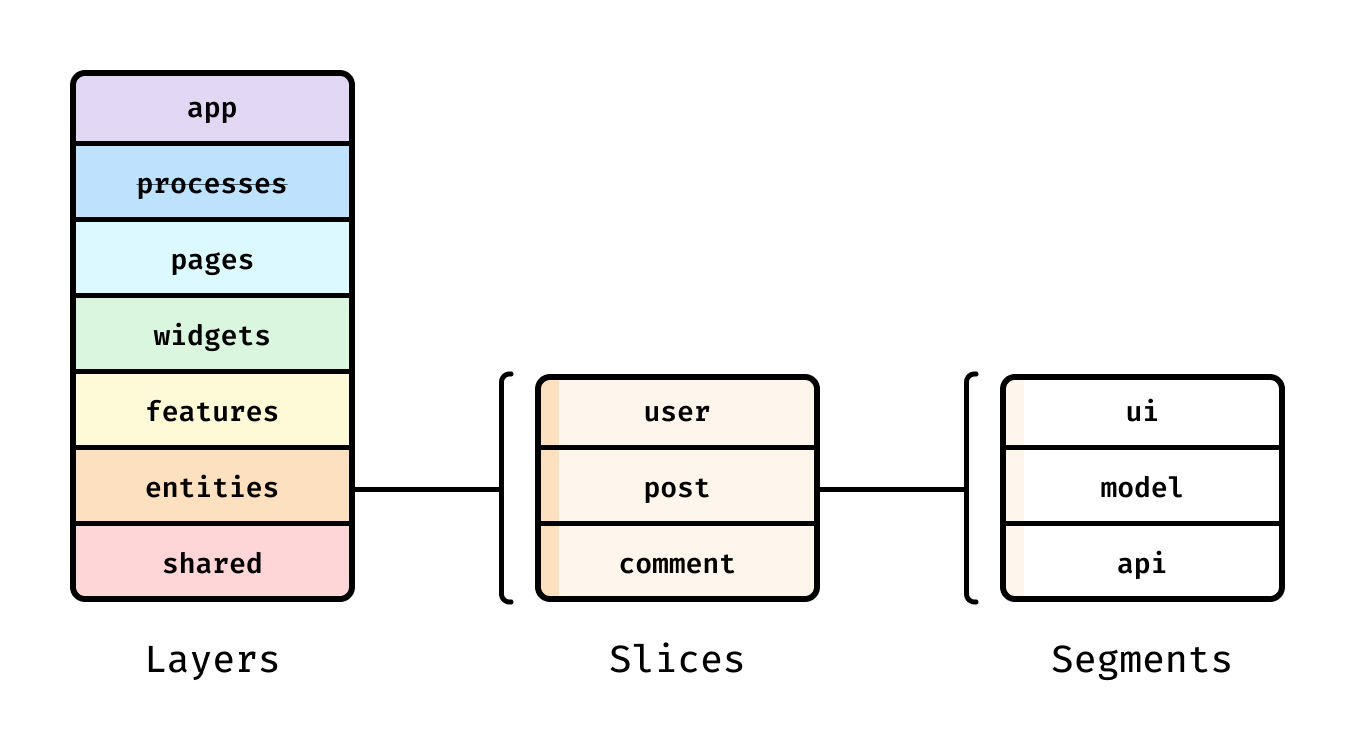
\includegraphics[width=0.7\linewidth]{static/fsdImage}
  \caption{Схема архитектуры клиентской части}
\end{figure}

На диаграмме представлены основные уровни и элементы архитектуры приложения. Следует отметить, что каждый слой в данной структуре ориентирован на строгое разграничение ответственности. Компоненты нижних уровней не имеют информации о вышестоящих слоях, что позволяет реализовать принцип инверсии зависимостей и минимизировать связанность между модулями.

\subsubsection{Слои архитектуры Feature-Sliced Design}

В таблице \ref{tab:fsd-layers} представлены слои архитектуры Feature-Sliced Design, сгруппированные по уровню абстракции и ответственности.

\begin{table}[h]
  \centering
  \caption{Слои архитектуры Feature-Sliced Design}
  \label{tab:fsd-layers}
  \begin{tabular}{|p{3cm}|p{11cm}|}
    \hline
    \textbf{Слой} & \textbf{Описание и назначение} \\ \hline
    \textit{app}      & Точка входа в приложение: глобальные стили, маршрутизация, провайдеры состояния, интеграции с внешними сервисами. \\ \hline
    \textit{pages}    & Страницы, связанные с маршрутизацией. Формируются из виджетов и не содержат бизнес-логики. \\ \hline
    \textit{widgets}  & Крупные элементы интерфейса, отражающие пользовательские сценарии, например, чат, список заданий, панель управления. \\ \hline
    \textit{features}& Изолированные пользовательские функции, такие как авторизация, отправка сообщений или регистрация. Могут включать бизнес-логику и вызовы API. \\ \hline
    \textit{entities} & Базовые предметные сущности предметной области, включающие типы, схемы, API и UI-представление. \\ \hline
    \textit{shared}   & Универсальные компоненты, утилиты и типы, переиспользуемые во всём проекте. \\ \hline
  \end{tabular}
\end{table}

\subsubsection{Концепция срезов}

Ключевым элементом архитектурного подхода Feature-Sliced Design является понятие срезов (англ. \textit{slices}). Под срезом понимается логически обособленный модуль, реализующий завершённую часть функциональности приложения. Каждый срез может содержать собственные модели данных, визуальные компоненты, бизнес-логику, а также механизмы взаимодействия с внешними источниками данных.

Ниже приведены примеры различных типов срезов и их ответственности в структуре проекта:

\begin{enumerate}
  \item \textit{features/login} — срез, реализующий сценарий авторизации пользователя;
  \item \textit{entities/task} — срез, содержащий всё, что связано с сущностью «задание»;
  \item \textit{widgets/ChatWindow} — срез, объединяющий функциональность и интерфейс чат-интерфейса;
  \item \textit{pages/home} — срез, реализующий главную страницу приложения.
\end{enumerate}

\subsubsection{Горизонтальное деление на сегменты}

Каждый срез, независимо от своего уровня, может быть дополнительно разделён на сегменты (англ. \textit{segments}) — логические подкатегории, структурирующие содержимое среза по назначению модуля. В отличие от слоёв, которые представляют вертикальную иерархию, сегменты формируют горизонтальное деление и обеспечивают внутреннюю организацию модулей.

Наиболее распространённые типы сегментов включают:
\begin{enumerate}
  \item \textit{ui} — визуальные компоненты и стили, определяющие отображение данных;
  \item \textit{model} — модели данных, хранилища состояния, типизация и бизнес-логика;
  \item \textit{api} — функции для работы с внешними сервисами, включая описание типов запросов и маппинг ответов;
  \item \textit{lib} — вспомогательные функции и библиотеки, используемые в пределах данного среза;
  \item \textit{config} — конфигурационные файлы и переключатели функциональности.
\end{enumerate}

\subsubsection*{Преимущества выбранного подхода}

Применение архитектуры Feature-Sliced Design в контексте разрабатываемого клиентского приложения позволило достичь следующих результатов:
\begin{enumerate}
  \item Чёткое разграничение обязанностей между модулями и слоями;
  \item Улучшенная масштабируемость проекта без деградации структуры;
  \item Повышенная модульность, обеспечивающая лёгкость в тестировании и повторном использовании текста программы;
  \item Создание условий для быстрой и эффективной интеграции новых членов команды в разработку;
  \item Архитектура, ориентированная на задачи и бизнес-логику, а не на технические детали.
\end{enumerate}

В совокупности данные свойства делают архитектурное решение устойчивым к росту функциональности, улучшая поддержку и развитие системы в долгосрочной перспективе.